\problem{}

1. Analyze the time complexities of the following algorithms and explain your reasoning.

\begin{algorithm}
\caption{}
\begin{algorithmic}
\For{$i \gets 1$ \textbf{to} $n$ \textbf{by} $i \gets 2i$}
    \For{$j \gets n$ \textbf{downto} $0$ \textbf{by} $j \gets j / 2$}
        \For{$k \gets j$ \textbf{to} $n$ \textbf{by} $k \gets k + 2$}
            \State $res \gets res + ij + jk$
        \EndFor
    \EndFor
\EndFor
\end{algorithmic}
\end{algorithm}


\begin{algorithm}
\caption{}
\begin{algorithmic}
\For{$i \gets n$ \textbf{downto} $0$}
    \For{$j \gets 1$ \textbf{to} $n$ \textbf{by} $j \gets 2j$}
        \For{$k \gets 0$ \textbf{to} $j$}
            \State $res \gets res + ij + jk$
        \EndFor
    \EndFor
\EndFor
\end{algorithmic}
\end{algorithm}

\noindent 2. Solve the following recurrence relations. Do not use the Master Theorem. Show all of your work.
$$T(n) = T(n-k) + 2k$$
$$T(n) = 2^kT(n/2^k) + kn$$
$$T(n) = 2^kT(n/2^k) + 2^k-1$$





\begin{figure}[htbp]
    \centering
    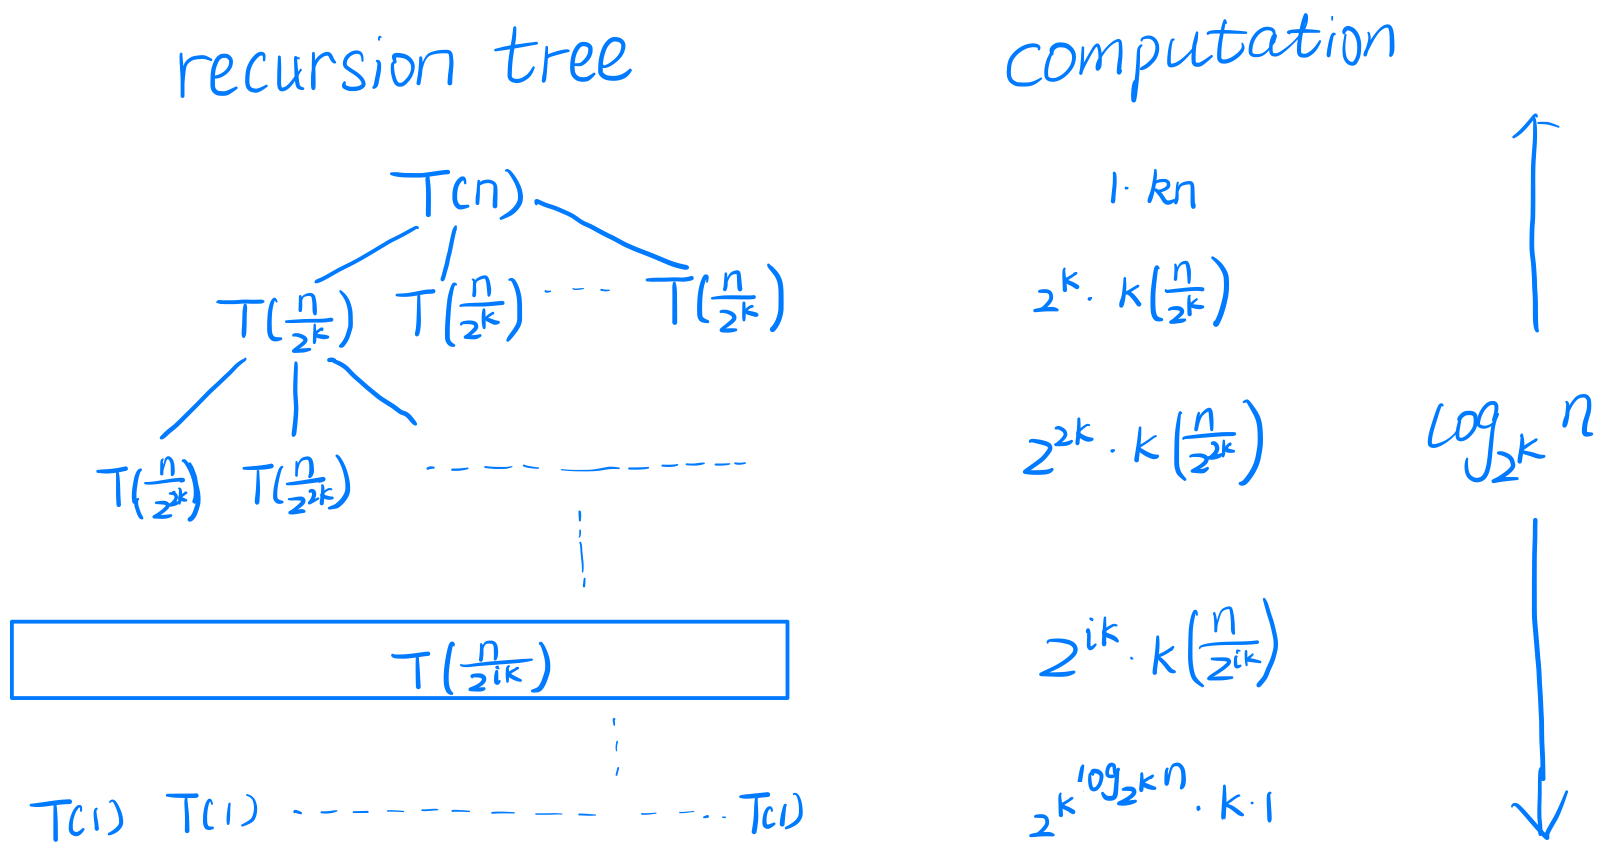
\includegraphics[width=0.9\linewidth]{./figure/t1_22.png}
    \caption{The recursion tree of $T(n) = 2^kT(n/2^k) + kn$}
    \label{fig:t1_22}
\end{figure}


\begin{figure}[htbp]
    \centering
    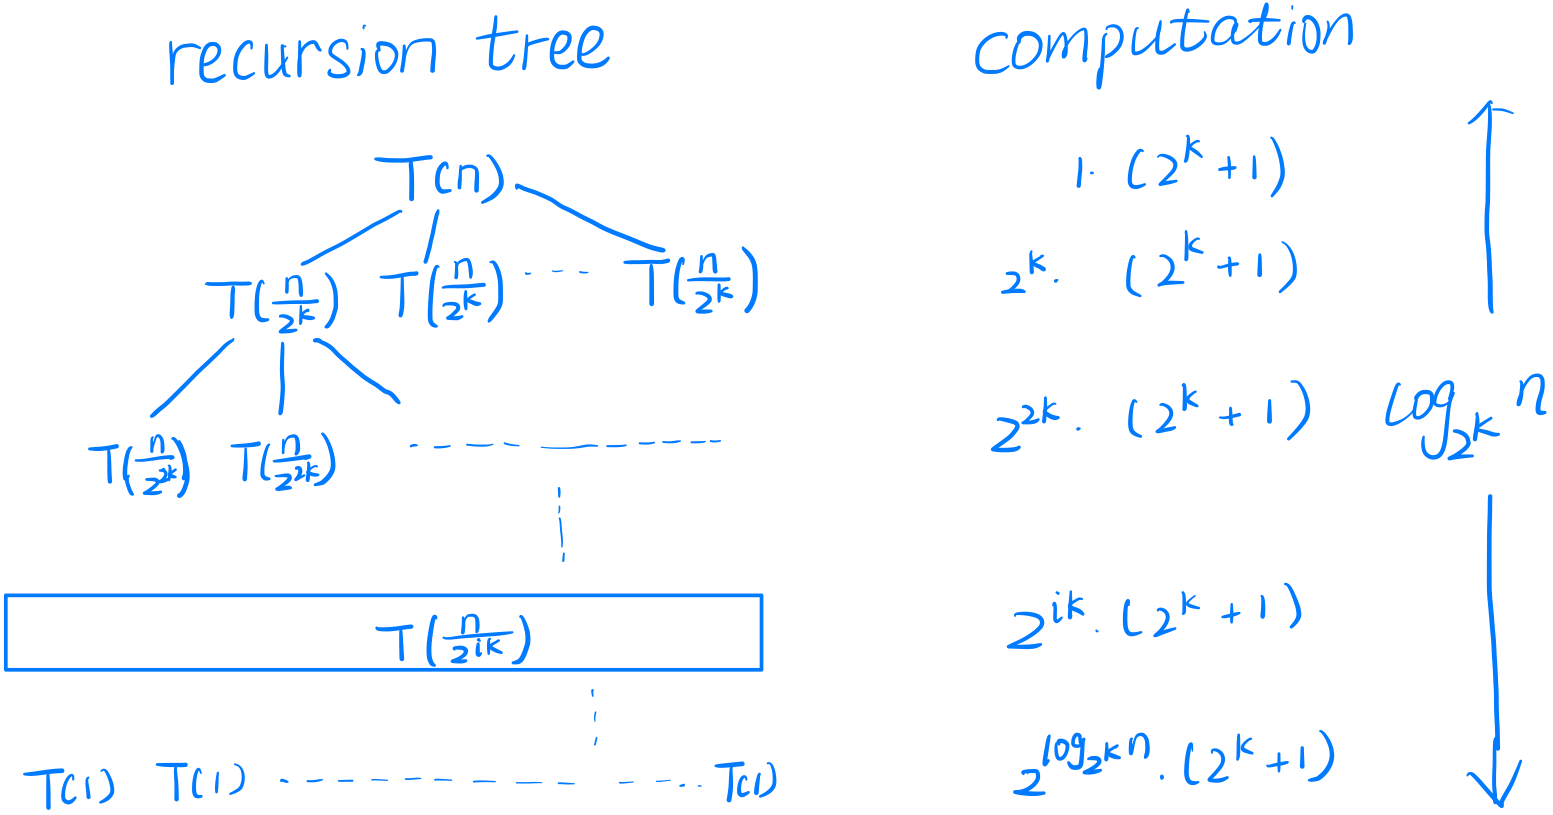
\includegraphics[width=0.9\linewidth]{./figure/t1_23.png}
    \caption{The recursion tree of $T(n) = 2^kT(n/2^k) + 2^k-1$}
    \label{fig:t1_23}
\end{figure}


\newpage